\documentclass{llncs}

\usepackage{booktabs}
\usepackage[ruled]{algorithm2e} % For algorithms

\usepackage{siunitx}
\usepackage{graphicx}
\usepackage{multirow}
\usepackage[caption=false]{subfig}
\usepackage[capitalise]{cleveref}
\usepackage{todonotes}

\begin{document}

\title{Audio Interface of an Active Perception Navigation Aid for People with Visual Impairments}
\titlerunning{Active Perception Interface for People with Visual Impairments}

\author{Jacobus C. Lock\inst{1} \and 
Iain Gilchrist\inst{2} \and
Grzegorz Cielniak\inst{1} \and
Nicola Bellotto\inst{1}}

\institute{University of Lincoln \email{\{jlock, gcielniak, nbellotto\}@lincoln.ac.uk} \url{https://lcas.github.io/ActiVis/} \and
	   University of Bristol \email{i.d.gilchrist@bristol.ac.uk}}

\authorrunning{Jacobus C. Lock et.\ al.}

\maketitle
\setcounter{footnote}{0}

\begin{abstract}
	%Our aim is to build a portable active navigation system for people with visual impairments that uses active perception techniques and a combination of feedback modes to identify a scene and guide a user to their destination.
	%Such a system requires a non-visual feedback interface and in this paper we investigate the effectiveness of a spatial audio tone with a varying pitch component, played through bone-conducting headphones, in conveying the pan and tilt angles of a target to the user in a pointing task.
	%The secondary goal is to determine how variations to the pitch's rate of change affect the user's performance.
	%For this, we conducted a set of experiments with both blindfolded participants and participants with visual impairments and found that, with some limitations, a spatialised audio tone with a varying pitch component can successfully convey a target's pan and tilt angles. 
  The ActiVis project is attempting to build a mobile guidance aid to help people with limited vision search for objects within an unknown environment.
  This system requires an effective non-visual interface to transmit guidance instructions to the user through means of bone-conducting headphones.
  To this end we propose a audio-based interface that uses a spatialised signal to convey a target's position on the horizontal plane. 
  The position on the median plan is given by adjusting the tone's pitch to overcome audio localisation issues that arise with bone-conducting headphones. 
  This interface is validated through a set of experiments. 
\keywords{Human-machine interface \and vision impairment \and spatialised sound \and varying pitch, pointing task}
\end{abstract} 

\section{Introduction}

In recent years, governments have spearheaded numerous initiatives to support people with disabilities and enable them to play a more active role in modern society.
The UK's Royal National Institute of Blind People (RNIB) for example has prioritised improving access to everyday services and products, such as public transport and mobile apps~\cite{rnib2016uk}.
Improvements in modern computing have made it possible for new and innovative solutions to these problems to come to the fore.
In particular, researchers in the active vision field have have made much progress in enabling machines to autonomously manipulate cameras to gather information about an environment for mapping and object and object finding tasks~\cite{bajcsy2018revisiting}.
There is, however, a significant research question about whether techniques from active machine vision can be applied to humans, i.e.\ can a machine identify a point of interest in a scene and direct a human, instead of an electronic servo, to focus on that point?
If this can be done, it would be beneficial to people with visual impairments and will augment their ability to search for an arbitrary point or object of interest and identify an unknown scene. 

The ActiVis project aims to deliver a mobile guidance system based on the Google Project Tango platform\footnote{\url{https://en.wikipedia.org/wiki/Tango\_(platform)}}, pictured in \cref{fig:tango-headphone}, that will ultimately be able to guide a user with vision impairments on the last leg of their journey, i.e.\ the so-called `last 10-yard problem'. 
The entire platform is based on a Google Project Tango device that provides access to powerful real-time localisation (through IMU measurements and landmark tracking) and image-processing facilities and provides access to Android's full range of interface tools and IO options. 
Furthermore, a set of bone-conducting headphones (pictured in \cref{fig:tango-headphone}) that are placed on a user's cheekbones instead of their ears and do not interfere with normal hearing, are used to transmit the audio signals to the user.
The system will provide real-time guidance instructions for the user to follow and it is important that these instructions are easily understood and are not perceived as a cognitive burden. 
Humans are naturally able to determine the 3D position of a sound source and by exploiting this ability, the system's guidance instructions can naturally be interpreted without posing a unnecessary burdensome cognitive load.
A sound source can be spatialised by adjusting a tone's spectral make-up (elevation angle), time delay and level difference (pan angle) and the intensity (distance).
Here only the pan and elevation positions are transmitted.
However, since bone-conducting headphones bypass the outer ear structure, their spectral signature cannot properly be interpreted and we therefore convey the target's elevation angle by simply adjusting the tone's pitch.

\begin{figure}[t]
  \centering
  \subfloat[]{\label{fig:tango-headphone}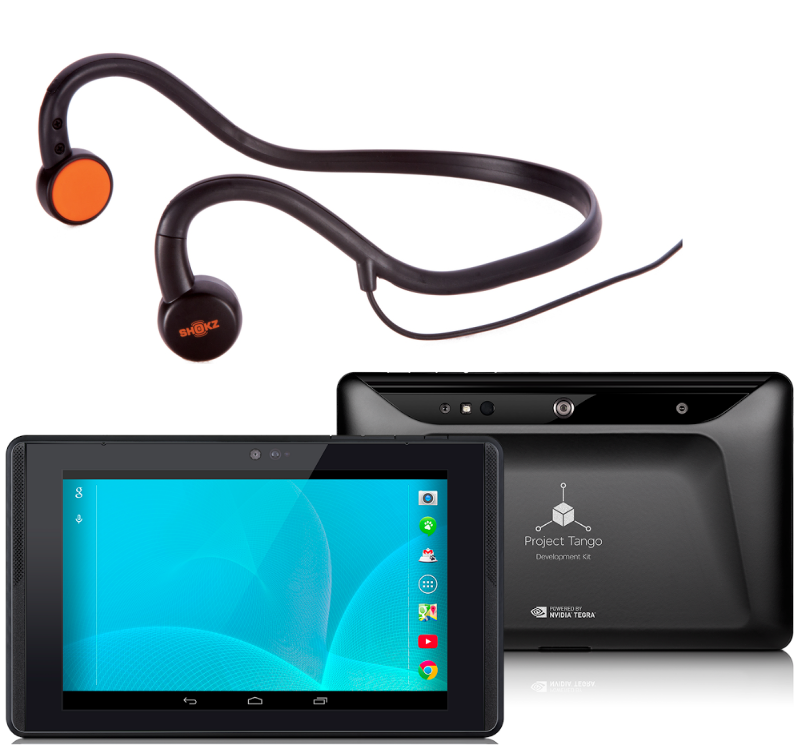
\includegraphics[width=0.4\columnwidth]{figures/tango_headphone.png}}
~
  \subfloat[]{\label{fig:participant}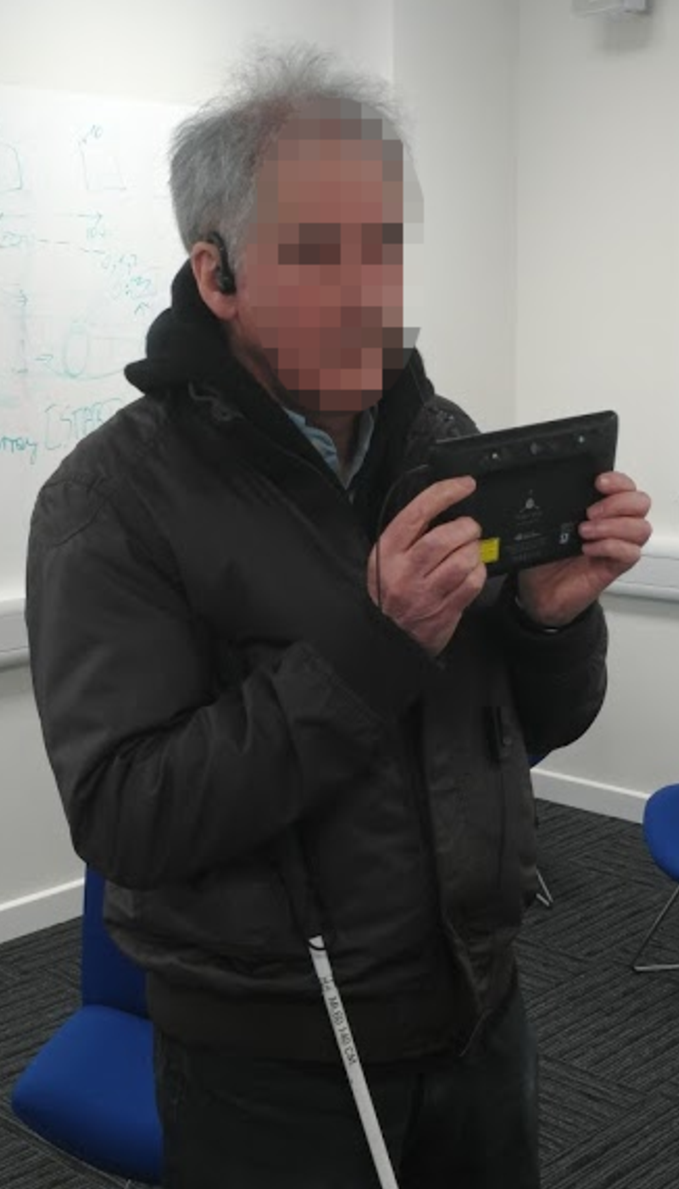
\includegraphics[width=0.25\columnwidth]{figures/vi_participant.pdf}}
  \caption{Pictures of the Tango device and bone-conducting headphones the system is based on (left) and both in use in an experiment (right).}
\end{figure}

A similar approach was used in\cite{durette2008visuo}, but the study did not focus on or investigate the interface's efficacy.
Indeed, this work serves as an initial study into an interface that can effectively communicate the pan and elevation angles of a target location through a set of bone-conducting headphones using a standard head-related transfer function (HRTF).
Furthermore, we demonstrate our approach's effectiveness through a simple experiment.
%The contribution of this work is an effective approach to addressing the shortcomings of playing spatialised sound through bone-conducting headphones, as well as initial experiments demonstrating its effectivenesst
%Furthermore, we demonstrate that such an interface is effective at communicating 

The rest of the paper is \todo{lay out rest of paper}

\section{Previous Work}

Work on guiding/directing people (vibration, audio, voice)
Show preference studies

Guidance instruction delivery modes using haptic, audio and vocal feedback for non-visual human-machine-interfaces (HMI) have been investigated before. 

Previous work on HRTF stuff

\todo{add previous work}

\section{Interface Description}

\subsection{Hardware Selection}

Electronic navigation aids and guidance systems for people with vision impairments have had trouble appealing to the visually impaired community at large because of problems that are typical of academic research and prototypes: prohibitive costs and user unfriendly interfaces and hardware requirements, e.g.\ head-mounted cameras and GPS antennae~\cite{golledge2004stated,yusif2016older,arditi2013user}.
Indeed, the traditional walking cane remains the go-to tool for navigation and obstacle avoidance. 
With the ActiVis system, we hope to tackle the issue of cost, user-acceptance and usability by using as many as possible `standard' devices and hardware as possible, with the idea that no specialist hardware is required and the user will not stand out if seen walking in public with a phone in their hand and wearing a headset.
The ActiVis system is based on a concept proposed in~\cite{bellotto2013multimodal,lock2017portable}, which uses a Google Tango device that is an Android-based device that comes equipped with an RGB-D camera to sense colour and depth and combines an inertial measurement unit (IMU) with powerful and robust landmark recognition and image processing algorithms to localise itself in real-time.
An benefit of such a platform is its familiar, compact form-factor which will help overcome the hurdle of user-acceptance and usability.

A set of bone-conducting headphones was selected as the audio transmission medium.
These headphones sit on a user's cheekbones and conduct the audio signals through the skull into the inner ear, instead of through the outer ear like typical over-ear headphones do. 
This has the benefit of not denying the user access to ambient sounds and noise, which could prove dangerous to a person with limited vision that relies on sound to detect oncoming vehicles and people, for example~\cite{lichtenstein2012headphone}.
Open-back headphones that allow ambient noise through were also considered, but the AfterShockz headphones pictured in \cref{fig:tango-headphone} were ultimately selected since they do not interfere at all with incoming sound (open-back headphones are better than closed back ones in this regard, but still muffle incoming sound) and are also more discreet than the larger over-ear headphone models. 

\subsection{Human Audio Localisation}

Humans localise a sound source in 3 dimensions by considering cues recorded in one ear (monaural cues) and comparing cues derived at both ears (binaural cues)\cite{blauert1997spatial,blauert1969sound}.
The binaural cues include time differences of arrival and intensity differences that help to determine a source's location on the horizontal plane.
Monaural cues are taken from the interaction of the sound with the human anatomy, e.g.\ head, shoulders, outer ear, before it enters the ear canal.
The user's anatomy acts as a filter and the direction the sound wave hits the body activates different filter resonances, attenuating or accentuating different frequency bands.
When the modified sound enters the inner ear, the human brain is able to analyse the frequency response and accurately determine the position of the sound source on the vertical plane. 
The distance to the source is simply derived as the intensity, or volume, of the source, i.e.\ a louder sound would appear closer to the user than a softer one does. 

When an audio signal is transmitted via a set of speakers or headsets, it can be transformed to mimic the characteristics of a natural sound sources before it is transmitted, thereby tricking the brain into believing a sound is located at some arbitrary position.
Such a transformation can be done using a head-related transfer function (HRTF) and a pair of stereo headsets or speakers.
An HRTF is a mathematical function that simulates the response signal of a human head and is derived by capturing key characteristics that affect the monaural and binaural responses, such as the user's hearing levels and head size, etc.
Since hearing responses can be quite unique between user's, the best results would be observed if each user had their own customised HRTF.\
Given the complicated process involved to capture the required user characteristics, making unique HRTFs is often an untenable solution and using average values (e.g.\ head measurements, height, etc.) have shown to produce acceptable results.\todo{cite HRTF papers}

\subsection{Interface Design}

The guidance target is presented to the user in terms of pan and elevation angles, indicating the angle adjustments that are required to point the device camera at the target location, as shown in \cref{fig:cam-coords}.
Spatialised audio signals are well-suited to the task, displaying similar levels of performance to vocal feedback, but with less cognitive load and higher resolution\cite{klatzky2006cognitive}.
However, the audio guidance signals are delivered to the user with a set of bone-conducting headphones that bypass the user's outer-ear structure and since this structure plays an important role in localising a sound source's elevation\cite{blauert1969sound}, an alternative mode of conveying the elevation angle is required.
For this work, we propose a simple linear adjustment to the signal's pitch as a function of the elevation angle. 
The pan angle can be conveyed by transforming the audio signal with an HRTF, and indeed it has been found that this dimension is unaffected by using bone-conducting headphones\cite{schonstein2008comparison,macdonald2006spatial,stanley2006lateralization}. 

\begin{figure}
  \centering
  \subfloat[]{\label{fig:cam-coords}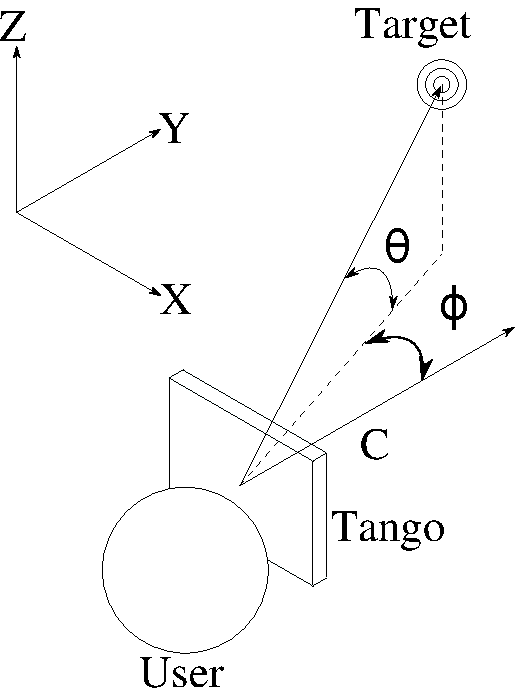
\includegraphics[width=0.3\columnwidth]{figures/camera_coordinate.pdf}}
~
  \subfloat[]{\label{fig:pitch-gain}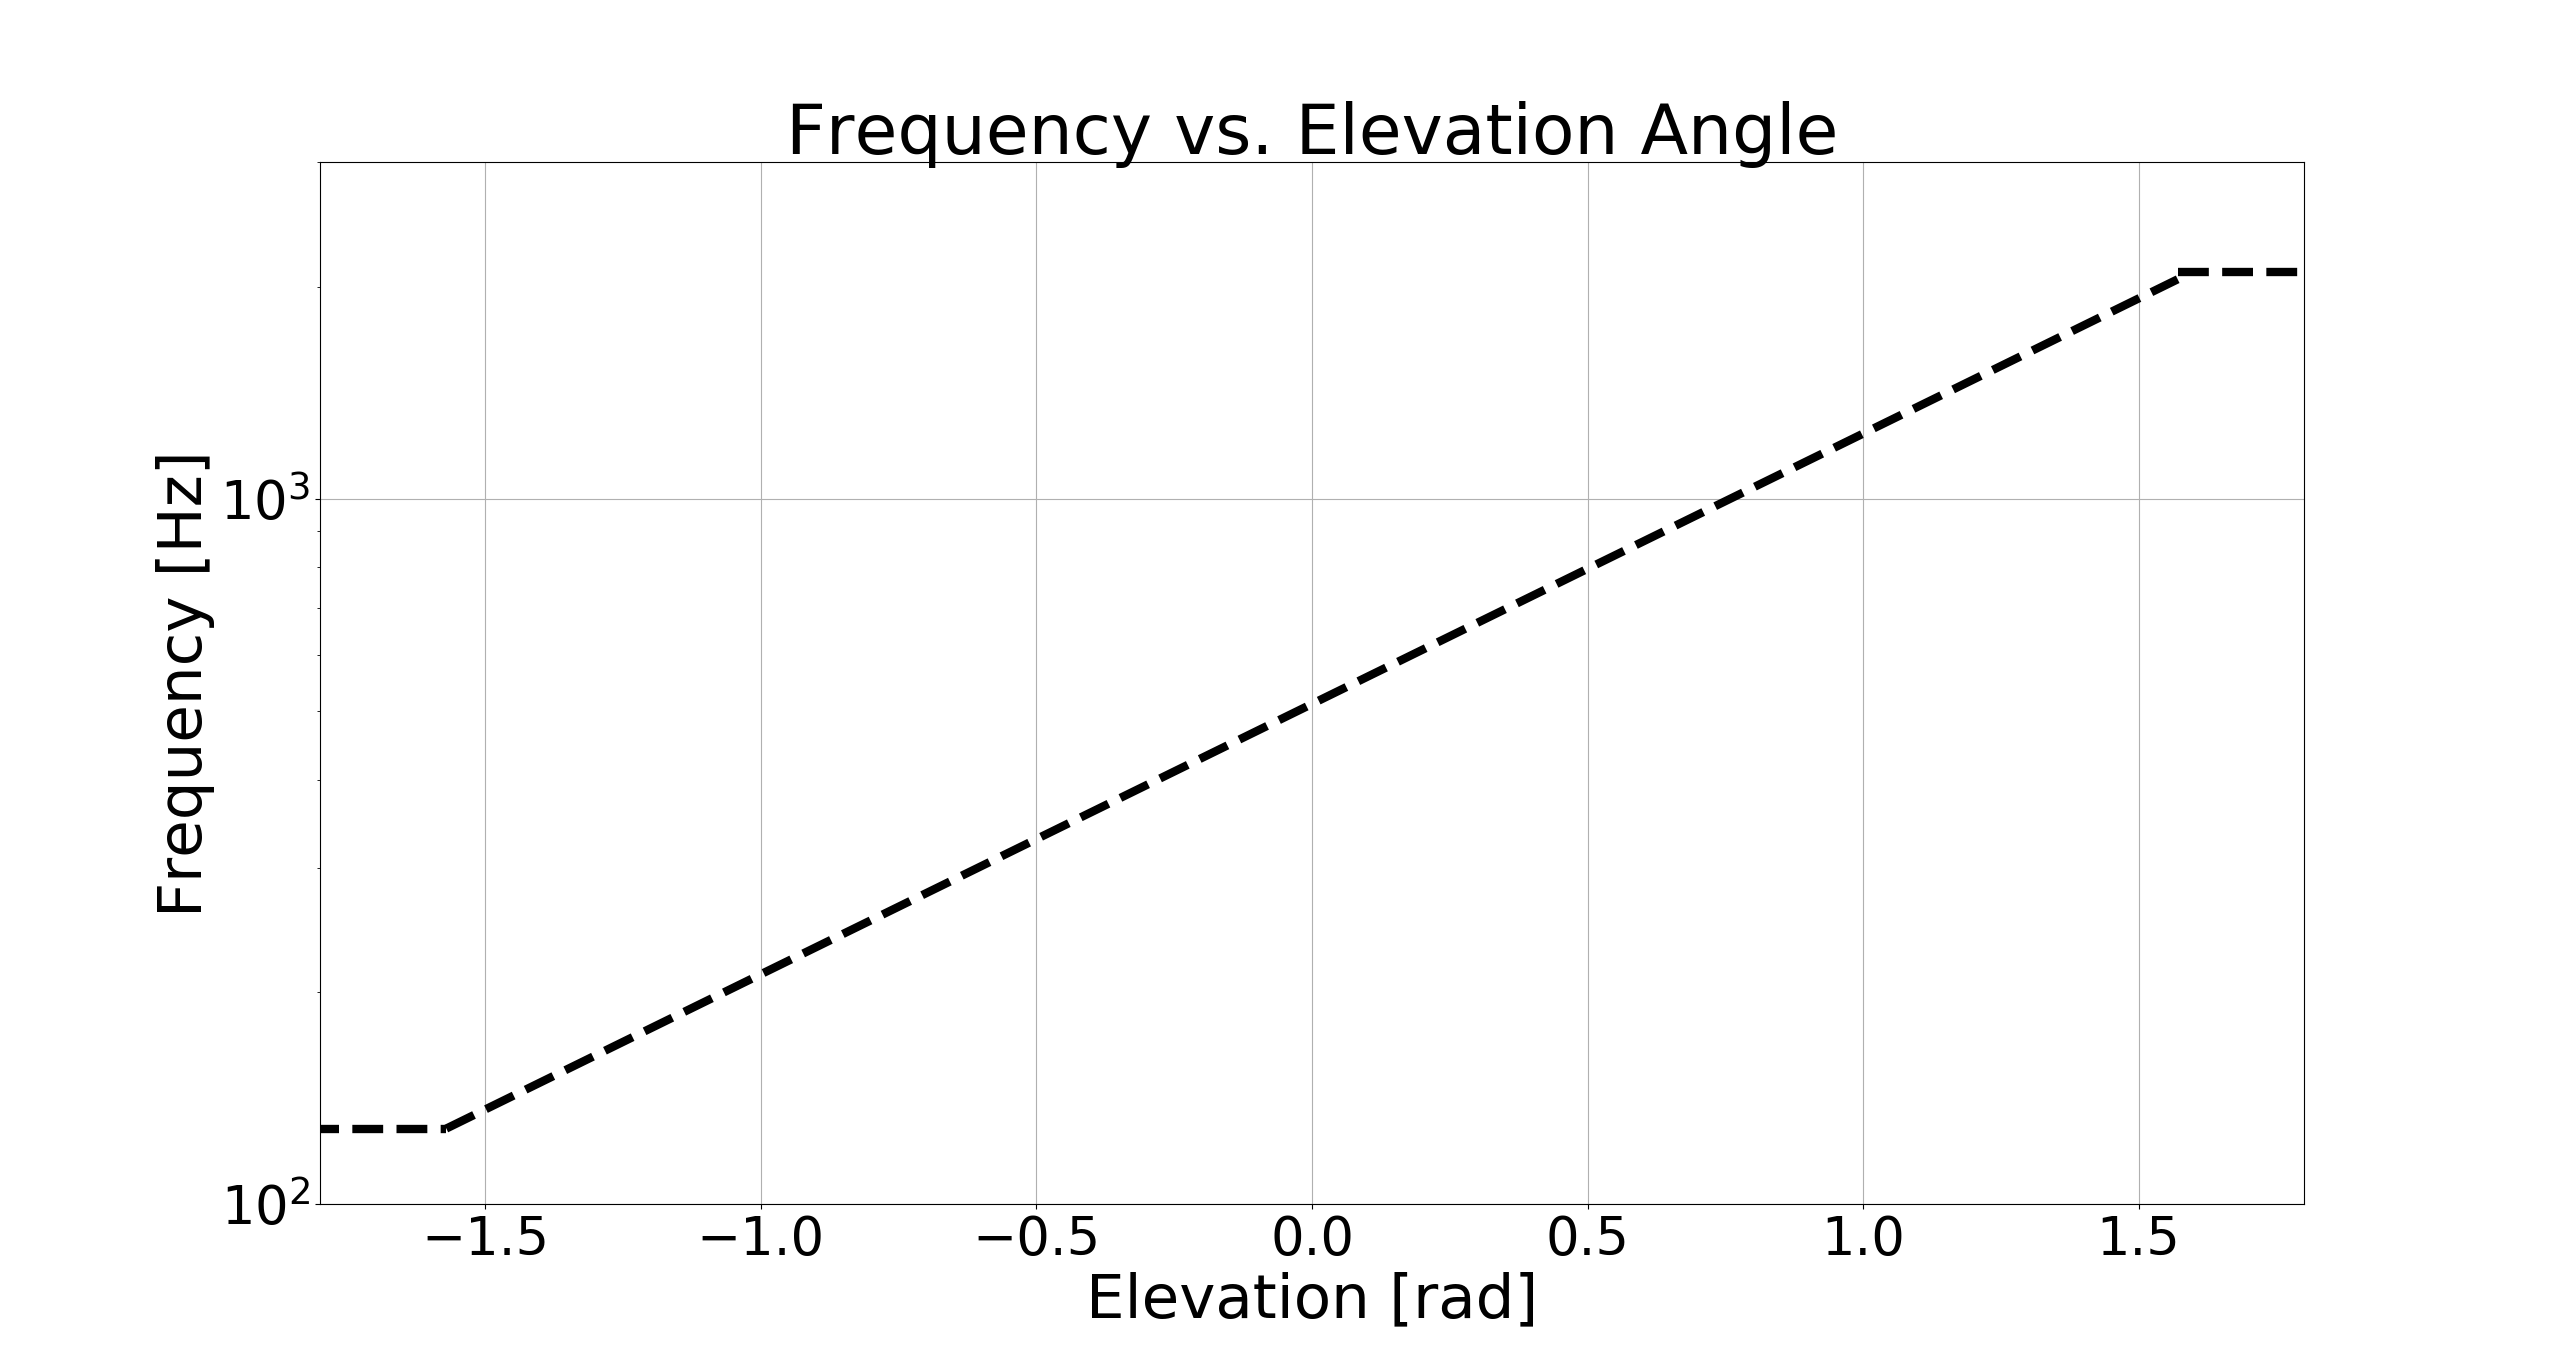
\includegraphics[clip, trim=0 0 0 40, width=0.6\columnwidth]{figures/pitch_gain_function.png}}
  \caption{The reference system used by the guidance interface showing the camera vector and pan and elevation angles (left) and the pitch gain function used to convey the target's elevation angle (right). }
\end{figure}

\subsubsection{Pan}

The human audition system uses binaural comparison cues, such as the inter-aural time and level differences (ITD and ILD respectively), to localise a sound source on the horizontal plane~\cite{blauert1969sound}.
The ITD is the perceived time delay between the signal reaching both ears, while the ILD is the perceived volume difference in the signal.
For example, a sound that comes from the individual's right, will hit the right ear first with a slightly higher volume.

In this work, a pure sinusoidal wave refreshed at \SI{10}{\hertz} was used. 
People typically have trouble localising a pure tone devoid of a rich spectral signature.
However, the ITD and ILD is independent of the tone's spectral make-up and the elevation angle is given through a different mechanism.
A pure sine wave is therefore sufficient to convey the target's pan angle.
To transform and spatialise the audio signal, we used OpenAL's default HRTF, based on the MIT's KEMAR dataset~\cite{hiebert2005openal,gardner1995hrtf}, that uses the user and targets' positions as input and outputs a transformed audio signal.

\subsubsection{Elevation}

Using a generic HRTF, such as OpenAL's KEMAR implementation, with bone-conducting headphones has been shown to have trouble conveying the elevation angle of a sound source accurately~\cite{macdonald2006spatial,schonstein2008comparison}.
To compensate for this, we convey the target's elevation angle by adjusting the tone's pitch (i.e.\ the sine wave's frequency) as a function of the elevation. 
When the camera vector is at the target's elevation, the tone is set to neutral pitch.
Then, when the target is above the camera vector, the pitch is increased and decreased when the target is below the camera vector.
This high/low association scheme is used given humans' natural association of high-pitched sounds with elevated sound sources and lower-pitched sounds with source's below the individual's earline~\cite{pratt1930spatial,blauert1997spatial}.
A logarithmic, octave and semi-tone based function is used to adjust the tone's pitch to ensure perceptible changes while keeping the timbre roughly constant~\cite{shepard1964circularity}.
The pitch is updated at a rate of \SI{10}{\hertz} and changes as the user moves the device.

The pitch is changed as a linear function of the elevation angle and the gradient is determined by setting the angle and pitch limits.
For this work we only consider a \SI{180}{\degree} field of view in front of the user and limit the elevation angle to a range of $[-\frac{\pi}{2}, \frac{\pi}{2}]$.
The pitch limits are set at some integer number of octaves above and below the neutral, on-elevation pitch.
After practical tests with the interface, we set the neutral pitch to \SI{512}{\hertz}, which is comfortably audible and allows for a large number of audible octave limits to be selected.
For this work, we set the pitch limits to 2 octaves away from the neutral pitch, giving frequency limits of [\SI{128}{\hertz}, \SI{2048}{\hertz}].
The linear function is visualised in \cref{fig:pitch-gain}.

\subsection{Implementation}

A diagram of the experimental system pipeline is shown in \cref{fig:pipeline}, where the arrows indicate the direction of the flow of information.
When the user taps the Tango's screen, a new virtual target is generated and its coordinates are sent to the audio generation module, along with the device's current position and orientation.
The audio generator then produces a tone based on the difference between the device and target's positions and sends it to the audio output channel, which plays it back to the user.
The WiFi recording module is constantly monitoring the different parameter values of the device and target's positions, as well as the system's output, and records it to a remotely stored datafile. 

\begin{figure}
  \centering
  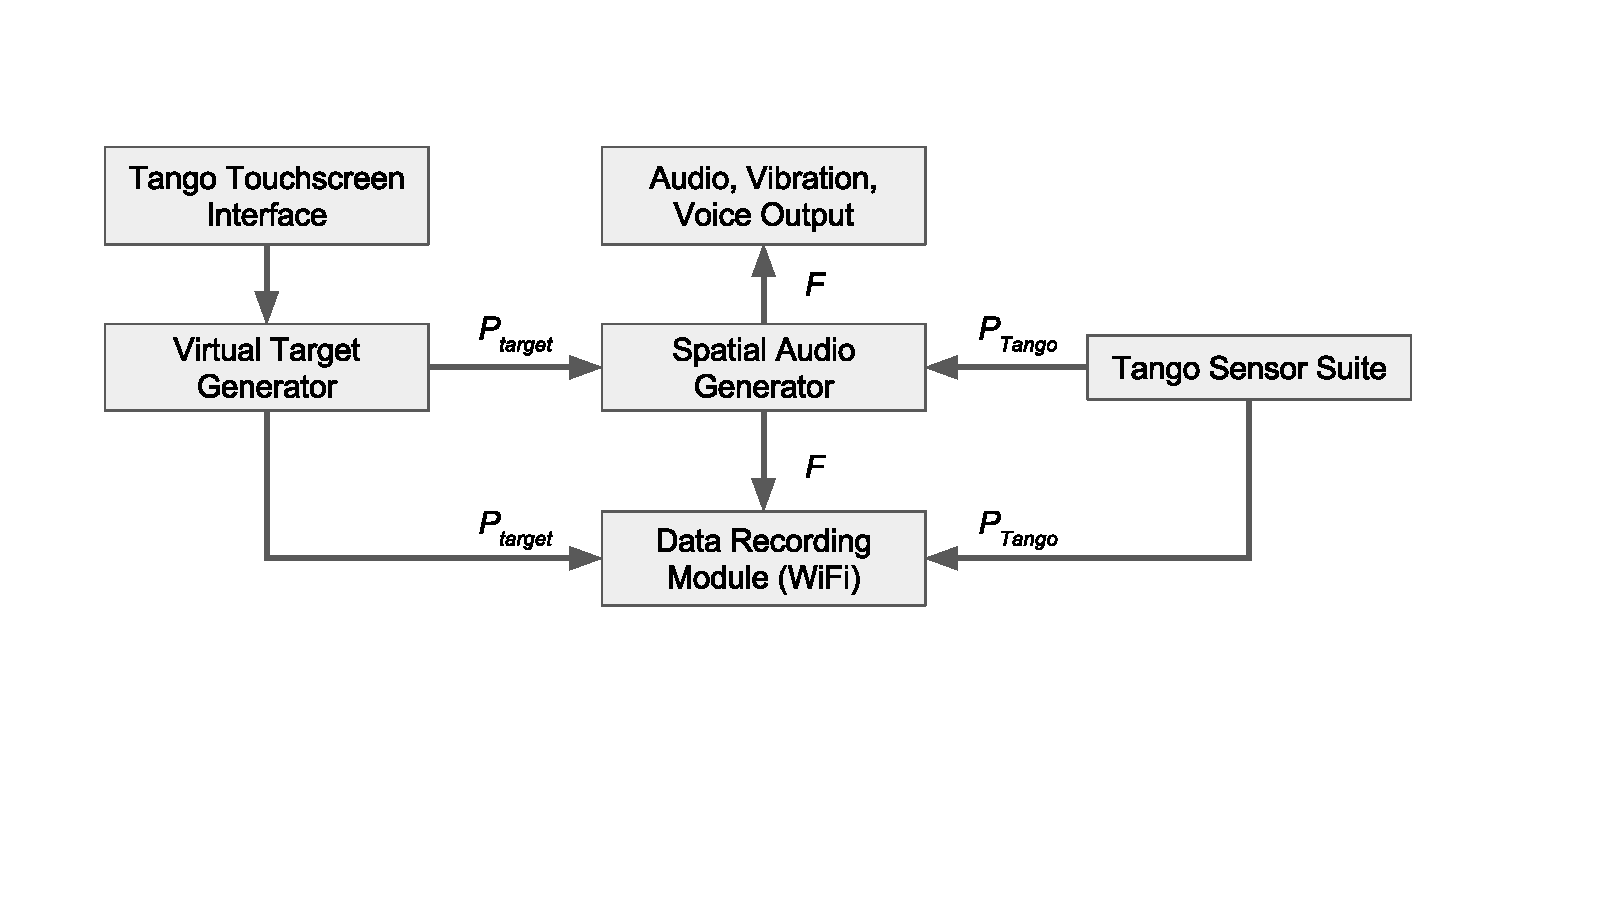
\includegraphics[clip=true, trim=0 120 80 50, width=0.8\columnwidth]{figures/pipeline.pdf}
  \caption{A diagram of the individual system components and their communication pipelines. $F$ indicates a feedback signal and $P$ a pose signal. }\label{fig:pipeline}
\end{figure}

\section{Experiment and Results}

To test the interface's effectiveness at directing a user towards a target area, a set of experiments were conducted with a simple pointing task. 
This pointing task is set up to capture the difference between the targets' actual position and the positions the participants' perceived them to be.

For the experiments, the participants are given a Tango tablet device running an app specifically written for these experiments. 
This app generates a set of virtual targets and presents them to the participants one at a time. 
The targets are generated at a constant \SI{2}{\meter} from the participant and their the pan and elevation angles are uniformly generated across 4 quadrants to avoid clustering.
Each target's angular position is communicated to the participant through the audio interface, the output of which is adjusted in real-time as the participant points the device around. 
When a participant was confident that they were on-target, i.e.\ hearing the audio front-on at \SI{512}{\hertz}, they tapped the screen, marking the location and generating the next target.
The targets' positions are all set relative to the Tango device's coordinate system which is tracked using the Tango localisation API.\
A total of 28 targets were generated per participant. 

2 groups of participants were recruited for the experiments. 
Group \textit{G1} consisted of 10 young adults with normal eyesight that were blindfolded for the experiments, and group \textit{G2} contains 4 people with severe vision impairments. 
Both groups were given some time with the system before the experiments commenced to familiarise themselves with the system, the audio signal's behaviour and the \SI{512}{\hertz} on-level tone. 
To minimise the speed/accuracy biases in the results, we asked the participants to focus on finding the targets as well as they could without worrying about the time it took.  

\subsection{Results}

The data collected during the experiment were grouped together by participant group and analysed.
Similar to the results from~\cite{macdonald2006spatial,schonstein2008comparison}, we use the absolute mean errors for each dimension which allows us to compare our results to the aforementioned works'. 
These results are presented in the boxplots in \crefrange{fig:sighted-err}{fig:blind-err} and summarised in \cref{tab:results}.

\todo{make plot text larger}
\todo{should we include blind results?}

\begin{figure}[t]
  \centering
  \subfloat[]{\label{fig:sighted-err}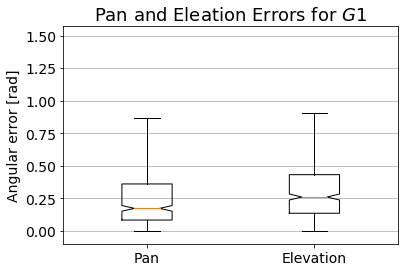
\includegraphics[width=0.5\columnwidth]{figures/pan_tilt_err_sight.png}}
~
  \subfloat[]{\label{fig:blind-err}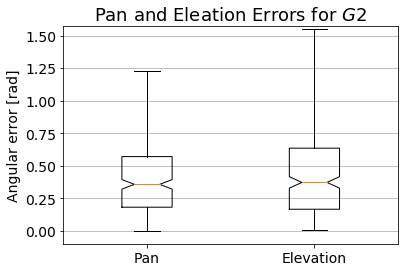
\includegraphics[width=0.5\columnwidth]{figures/pan_tilt_err_blind.png}}
  \caption{Boxplots of the angular errors collected during the pointing experiment for the blindfolded (left) and visually impaired (right) participants. }
\end{figure}

\begin{table}
  \centering
  \caption{}\label{tab:results}
  \begin{tabular}{p{1cm}cc}
    \toprule
	                         &           & Mean absolute error [rad] \\ \midrule
    \multirow{2}{*}{\textit{G1}} & Pan       & $ 0.25\pm0.24$ \\
				 & Elevation & $ 0.37\pm0.27$ \\ \midrule
    \multirow{2}{*}{\textit{G2}} & Pan       & $ 0.48\pm0.33$ \\
				 & Elevation & $ 0.58\pm0.42$ \\
    \bottomrule
  \end{tabular}
\end{table}

\todo{add correlation plots}

The average pan error from group \textit{G1} falls well within the ranges observed in~\cite{macdonald2006spatial,schonstein2008comparison} of $[0.16, 0.38]$ radians and $[0.17, 0.26]$ radians respectively. 
Indeed, the majority of samples fall within even the more conservative latter range. 
However, the participants with vision impairments in group \textit{G2}  demonstrate a wider spread in error data and higher average error than \textit{G1} (0.23 vs. 0.40 radians, Kruskal-Wallis test $p=0.05$). \todo{do KW test}
The results in~\cite{katz2011spatial,zwiers2001spatial} reported a similar trend, but an investigation with a larger sample size for \textit{G2} should be considered before definitive conclusions can be made.

The elevation estimation performance for both groups deteriorated when compared to their pan estimation results, which was somewhat expected given previous research results on human audition. \todo{cite vertical vs horizontal performance}
The mean absolute errors of the participants are \SI{0.37}{\radian} and \SI{0.58}{\radian} for groups \textit{G1} and \textit{G2} respectively.
Comparing these results to methods that convey elevation through an HRTF, we see an improvement of approximately 46\% and 16\% for each group~\cite{schonstein2008comparison}. 
There is a lesser improvement (13\%) with \textit{G1} when compared to the individualised and adjusted HRTFs in~\cite{stanley2006lateralization} and a 13\% reduction in performance for group \textit{G2}.
However, the participants from~\cite{stanley2006lateralization} all had healthy eyesight, making the latter comparison invalid. 
Interestingly, the elevation errors for group \textit{G2} is centered around the negative angle, indicating a possible underlying bias in the participants or the interface.
A similar trend was observed in~\cite{stanley2006lateralization} and warrants an investigation with a larger participant pool to determine the underlying bias, if any. 

\section{Conclusion}

In this work, we proposed an audio interface that conveys a target's pan and elevation angles through a spatialised audio tone that adjusts the tone's pitch to convey the elevation in compensate for the shortcomings of bone-conducting headsets in transmitting the elevation component of a spatialised signal.
Results generated from a simple pointing experiment are encouraging and improves performance over purely spatialised signals transmitted via bone-conduction.
Future work will involve a more in-depth investigation with a larger participant pool to determine the factors that affect performance and enable a more detailed statistical analysis.
For example, will adjusting the elevation function's gradient make it easier to guess the target's elevation and what is the performance difference between participants with limited and healthy eyesight?  

%\section{Previous Work}\label{sec:lit-review}

%Earlier attempts at improving a person with visual impairment's navigation experience involved outfitting the commonly-used walking cane with remote detection systems, such as sonar, radar and RFID tags, to transform a cane into an early-warning system~\cite{ulrich1997,marion2008batcane,faria2010electronic,willis2005}.
%Bluetooth tags and a smartphone can be used in a similar manner~\cite{sato2017navcog3}.
%However, the expense and effort of maintaining such tags make them less attractive for wide-scale adoption.
%Computer vision-based systems provide a good compromise between usability, cost and accuracy.
%One solution is to use RGB-D depth sensing cameras, which are becoming increasingly accurate and cost-effective, to build a 3D image map of the environment, and guiding a user through it~\cite{lee2015,rodriguez2012obstacle}.
%Alternatively, object recognition techniques can be used to detect various objects and landmarks, such as doors, staircases, etc., and communicate their relative location to the user~\cite{schauerte2012assistive,tian2013b,fiannaca2014headlock}, or use audio instructions to guide a user to fully capture an object of interest~\cite{vazquez2012helping}. 

%An important feature of user-centric systems is a human-machine interface (HMI) that enables effective two-way communication between the system and the user.
%Surveys found that people with visual impairments prefer receiving instructions in the form of speech and haptic feedback cues~\cite{khoo2016multimodal,ross2000wearable,vazquez2012helping}.
%However, haptic feedback modes typically have a lower bandwidth when compared to audio feedback and also require the user to wear a special device in order to transmit the signals effectively.
%Work has also been done in translating a visual scene into non-visual formats, with so-called sensory substitution systems (e.g. `The Voice'~\cite{meijer2010}) and virtual audio reality (VAR) systems~\cite{frauenberger2003} reporting favourable results.
%However, The Voice has a very steep learning curve that has proven to be a significant barrier to entry and with VAR systems, it is not clear how unknown environments, where markers have not yet been encoded, would be handled and described to the user. 

%Previous experiments have determined that people are able to find the location of a stationary sound source with an error of $\pm$\SI{35}{\degree}, in both the pan and tilt dimensions~\cite{zwiers2001spatial}, for both early-blind and normally-sighted people.
%However, in~\cite{lewald2013exceptional,lessard1998early} it was found that the blind have a clear advantage in localisation accuracy over sighted people when presented with more complex tasks, such as targets in motion and narrow-band stimuli, with~\cite{lewald2013exceptional} reporting an average absolute localisation error of around \SI{10}{\degree} in the pan and tilt dimensions.
%Researchers have used simulated spatialised audio to inform the user of the sound source's direction~\cite{holland2002audiogps,kammoun2012navigation,rebillat2009smart,menelas2010audio,wilson2007swan,zotkin2004rendering}.
%In these works, a sound was played through a set of headphones and the source spatialised with a head-related transfer function (HRTF), tricking the listener into thinking the sound source was located at some arbitrary 3D location.
%There are also experimental results about how well users can find targets presented with spatial sound in the tilt and panning dimensions with normal headphones~\cite{katz2011spatial,zwiers2001spatial}, as well as work that has shown similar levels of localisation performance between normal and bone-conducting headphones in the pan dimension~\cite{macdonald2006spatial}.
%However, to our knowledge no extensive work or experiments have been done to determine how well users respond to tilt adjustment instructions using a tone with \textit{varying pitch}, in particular when using bone-conducting headphones, and how changes to this tone's behaviour affects performance. 

%\section{Conclusion and Future Work}\label{sec:conclusion}

%In this work, we present an audio-based guidance interface that uses a spatialised audio tone with varying pitch to direct a user with visual impairments to point a camera toward a target. 
%We also present and discuss a set of experiments that were conducted to determine the interface's effectiveness and performance, as well as some subjective feedback that was collected from legally blind participants. 

%Using a set of bone-conducting headphones, we found that a spatialised audio tone with a varying pitch can successfully convey the pan and tilt angles of a target.
%The angular errors made by the participants are in line with those from previous research using similar audio guidance instructions.
%We also found that varying the pitch's rate of change influences the accuracy of the system in the tilt dimension without affecting the performance in the pan dimension.
%The steeper, $m_h$ and $m_m$ pitch gradients were found to produce the best accuracy results in general.

%Feedback from the participants with visual impairments was mostly positive and they agreed with the choice of bone-conduction headphones that do not inhibit normal hearing.
%However, they noted that the sine wave audio signal induced audio fatigue after extended exposure, something noted by the other participants as well, and suggested that more full-bodied, natural sounds be used instead.
%Using vocal feedback in conjunction with the current audio signal was also suggested. 

%These results are more interesting from a design point of view than an end-user's. 
%Indeed, we have shown that this audio guidance interface is effective at directing an average person, but more data are needed with the intended audience in order to decisively conclude that this interface will be effective in an indoor guidance system for people with vision impairments. 
%Nevertheless, these data are a good indication of what to expect when we evaluate this audio interface with a greater number of people with limited vision.
%Once we have determined that the intended audience can effectively use this type of guidance instruction, we can start adding more user-oriented features (e.g.\ voice prompts, more pleasant tones, etc.) and integrate them into our guidance system prototype. 

\bibliographystyle{splncs04}
\bibliography{bib}

\end{document}
